% debut d'un fichier latex standard
\documentclass[a4paper,12pt,twoside]{article}
% Tout ce qui suit le symbole "%" est un commentaire
% Le symbole "\" désigne une commande LaTeX

% pour l'inclusion de figures en eps,pdf,jpg, png
\usepackage{graphicx}

% quelques symboles mathematiques en plus
\usepackage{amsmath}

% le tout en langue francaise
%\usepackage[francais]{babel}

% on peut ecrire directement les caracteres avec l'accent
%    a utiliser sur Linux/Windows (! dépend de votre éditeur !)
%\usepackage[utf8]{inputenc} % Pour TeXworks
%\usepackage[latin1]{inputenc} % Pour Kile
%\usepackage[T1]{fontenc}

%    a utiliser sur le Mac ???
%\usepackage[applemac]{inputenc}

%-----------------------------------------------------------------------------------------------------------------
% Choix du bon package en fonction de la compilation
% ----------------------------------------------------------------------------------------------------------------

\usepackage[francais]{babel} %indique qu'on veut travailler en francais, en r�glant les accents, les espaces ins�cables, etc. automatiquement
\usepackage{iftex}

\ifPDFTeX
	\usepackage[utf8]{inputenc} %input encoding
	\usepackage[T1]{fontenc} %font encoding with pdflatex
	\usepackage{lmodern}
\else
	\ifXeTeX
		\usepackage{fontspec} %input encoding
	\else 
		\usepackage{luatextra}
	\fi
	\defaultfontfeatures{Ligatures=TeX}
\fi

% pour l'inclusion de liens dans le document 
\usepackage[colorlinks,bookmarks=false,linkcolor=black,urlcolor=blue, citecolor=black]{hyperref}

\paperheight=297mm
\paperwidth=210mm

\setlength{\textheight}{235mm}
\setlength{\topmargin}{-1.2cm} % pour centrer la page verticalement
%\setlength{\footskip}{5mm}
\setlength{\textwidth}{16.5cm}
\setlength{\oddsidemargin}{0.0cm}
\setlength{\evensidemargin}{-0.3cm}

\pagestyle{plain}

% nouvelles commandes LaTeX, utilis\'ees comme abreviations utiles
\def \be {\begin{equation}}
\def \ee {\end{equation}}
\def \dd  {{\rm d}}

\newcommand{\mail}[1]{{\href{mailto:#1}{#1}}}
\newcommand{\ftplink}[1]{{\href{ftp://#1}{#1}}}
%
% latex SqueletteRapport.tex      % compile la source LaTeX
% xdvi SqueletteRapport.dvi &     % visualise le resultat
% dvips -t a4 -o SqueletteRapport.ps SqueletteRapport % produit un PostScript
% ps2pdf SqueletteRapport.ps      % convertit en pdf

% pdflatex SqueletteRapport.pdf    % compile et produit un pdf

% ======= Le document commence ici ======

\begin{document}

	% Le titre, l'auteur et la date
	\title{Particule charg\'ee dans un champ \'electromagn\'etique}
	\author{Coppex Aur\'elie H\'el\`ene, Ventura Vincent\\  % \\ pour fin de ligne
	{\small \mail{aurelie.coppex@epfl.ch, vincent.ventura@epfl.ch}}}
	\date{\today}\maketitle
	\tableofcontents % Table des matieres

	% Quelques options pour les espacements entre lignes, l'indentation 
	% des nouveaux paragraphes, et l'espacement entre paragraphes
	%\baselineskip=16pt
	%\parindent=0pt
	%\parskip=12pt



\section{Introduction} %------------------------------------------

	Dans le domaine de la physique, il est possible de d\'ecrire de nombreux phénomènes du monde. Pour cela, il est souvent n\'ecessaire de recourir au calcul num\'erique pour r\'esoudre des \'equations qui ne peuvent pas \^etre calcul\'ees analytiquement. Il existe plusieurs m\'ethodes pour les r\'esoudre, dont les int\'egrateurs. Il faut cependant savoir les choisir en fonction du probl\`emes trait\'es et pour cela, il faut les conna\^itre.

	Dans cet exercice, il est question d'une particule charg\'ee dans un champ \'electromagn\'etique subissant une force de Lorentz. 
	
	Le but est d'en \'etudier la trajectoire afin de pouvoir analyser les propri\'et\'es de stabilit\'e et de convergence des cinq sch\'emas suivants : 
	Euler explicite, Euler implicite, Euler-Cromer, Runge-Kutta d'ordre 2 et Boris Buneman \cite{NdC}.
	\newpage

\section{Calculs analytiques}

	Dans cette partie, tous les calculs sont faits avec les valeurs suivantes :
	
	la masse de la particule : $m = 1.6726 \cdot 10^{-27}$ kg, 
	
	la charge de la particule :	$q = 1.6022 \cdot 10^{-19}$ C ,
	
	sa position initiale : $\vec{v_0} = (v_{x0}, v_{y0})$.
	
	La particule est plongée dans un champ \'electrique uniforme $\vec{E} = E_0 \hat{z}$ et un champ magn\'etique uniforme $\vec{B} = B_0 \hat{y}$.


	\subsection{\'Equations du mouvement}
	
		On cherche tout d'abord \`a \'etablir les \'equations diff\'erencielles du mouvement sous la forme $\frac{d\bf y}{dt} = {\bf f(\bf{y}})$ avec ${\bf y} = (x, z, v_x, v_z)$. 
		Pour cela, on applique la $2^{eme}$ loi de Newton ($\sum{\bf F} = m \bf a$ ) et on la projette sur les axes x, y et z.
		
		Il en r\'esulte :
		
		\begin{equation}
			{\bf F_p  + F_L} = m \bf{a}
		\end{equation}
		
		Avec ${\bf F_p}$, la force de pesanteur et ${\bf F_L}$, la force de Lorentz.
		
		La force de pesanteur est n\'egligeable pour une particule \'el\'ementaire. Il ne reste donc que la force de Lorentz qui est donn\'ee par : $\vec{F} = q(\vec{E}+\vec{v} \times \vec{B})$.
		
		Les projections sur les axes donnent:
		
		\begin{equation}\label{xpp}
			{\bf(Ox):} -qB_0 \dot{z} = m \ddot{x}  \iff \ddot{x} = -\frac{qB_0}{m} \dot{z}
		\end{equation}
		
		\begin{equation}
			{\bf(Oy):}  0 = m \ddot{y} \iff \ddot{y} = 0
		\end{equation}
		
		\begin{equation}\label{zpp}
			{\bf(Oz):}  q(E_0 + B_0\dot{x}) = m \ddot{z} \iff \ddot{z} = \frac{q}{m} (E_0+B_0 \dot{x}) 
		\end{equation}
		
		L'\'equation du mouvement s'\'ecrit donc :
		\begin{equation}
		\frac{d\bf y}{dt} = \begin{pmatrix}  \dot x \\ \dot z \\ -\frac{qB_0}{m} \dot{z} \\ \frac{q}{m} (E_0+B_0 \dot{x}) \end{pmatrix}
		\end{equation}
		

	\subsection{\'Energie m\'ecanique et sa conservation}
	
		L'\'energie m\'ecanique est d\'efinie comme : $E_{mec} = E_{cin} + E_{pot}$. Or, l'\'energie cin\'etique est connue et vaut $E_{cin} = \frac{1}{2} m {\vec{v}}^2$.
		Il ne reste donc plus qu'\`a calculer l'\'energie potentielle. Pour cela, la formule $E_{pot} = \int_P^O \vec{F}\, \mathrm d\vec{l}$ \cite{FT}. Ce qui donne :
	
			\begin{equation}
				E_{pot} = qE_0 (z_0-z)
			\end{equation}
		
		Ainsi, l'\'equation suivante est obtenue :
	
			\begin{equation}
				E_{mec} = \frac{1}{2}m(v_x^2+v_z^2) + qE_0(z_0 - z)
			\end{equation}
		
		Pour montrer que cette \'energie est conserv\'ee, il faut en calculer la d\'eriv\'ee:
	
			\begin{equation}
				\frac{dE_{mec}}{dt} = \frac{1}{2} m(2\dot{x}\ddot{x} + 2\dot{z}\ddot{z}) - 	qE_0\dot{z} 
			\end{equation}
		En appliquant les équations (\ref{xpp}) et (\ref{zpp}), on trouve:
	
			\begin{equation}
				\frac{dE_{mec}}{dt}= -qB_0\dot{z}\dot{x}+qE_0\dot{z}+qB_0\dot{x}\dot{z}-qE_0\dot{z} = 0
			\end{equation}
	
		Ce qui prouve que l'\'energie m\'ecanique est conserv\'ee.
	
	\subsection{Solution analytique}
	
		Les conditions initiales sont les suivantes : $\vec{x}(0) = 0$ et $ \vec{v}(0) = v_0\hat{z}$.
		
		En int\'egrant les \'equations (\ref{xpp}) et (\ref{zpp}), il est possible de trouver $\dot{x}$ et $\dot{z}$ :
		
			\begin{equation}\label{aa}
				\left \{
				\begin{array}{r c l}
					\dot{x} & = & -\frac{qB_0}{m}z + C_1  \\
					\dot{z} & = & \frac{q}{m} (E_0t + B_0x) + C_2\\
				\end{array}
				\right .
			\end{equation}
		
		En appliquant la condition initiale $ \vec{v}(0) = v_0\hat{z}$ à (\ref{aa}), on obtient $C_1 = \frac{qB_0}{m}z_0 $ et $C_2 = v_0 -\frac{q}{m}B_0x_0$.

			
		En les appliqant dans les \'equations de la vitesse, il en ressort :
				
			\begin{equation}\label{v}
				\left \{
				\begin{array}{r c l}
					v_x(t) & = & \frac{qB_0}{m}(z_0 - z)\\
					v_z(t) & = & v_0 + \frac{qB_0}{m}(x-x_0) + \frac{qE_0}{m}t\\
				\end{array}
				\right .
			\end{equation}
			
		\`A partir desquelles (\ref{v}) il est possible de trouver les \'equations de l'acc\'eleration:
		
			\begin{equation} \label{diff}
				\left \{
				\begin{array}{r c l}
					\ddot{x} - \frac{q^2B_0^2}{m^2}x & = & \frac{q^2B_0E_0}{m^2}t-\frac{qB_0 }{m}v_0 - \frac{q^2B_0^2}{m^2}x_0\\
					
					\ddot{z} -\frac{q^2B_0E_0}{m^2}z& = &  \frac{qE_0}{m} -\frac{q^2B_0E_0}{m^2}z_0\\
				\end{array}
				\right .
			\end{equation}
	
	En r\'esolvant les \'equations diff\'erentielles du 2\`eme ordre (\ref{diff}), on trouve la solution analytique suivante :
	
		\begin{equation} 
			\left \{
			\begin{array}{r c l}
				x(t) & = & \frac{qB_0v_0}{m} \cos(\frac{m}{qB_0}t) + \frac{E_0m}{qB_0^2} \sin(\frac{qB_0}{m}t) -\frac{E_0}{B_0}t - \frac{mv_0}{qB_0} \\
				v_x(t) & = & - v_0 \sin(\frac{qB_0}{m}t) + \frac{E_0}{B_0} \cos(\frac{qB_0}{m}t) -\frac{E_0}{B_0} \\
				z(t) & = & -\frac{mE_0}{qB_0^2} \cos(\frac{qB_0}{m}t) + \frac{mv_0}{qB_0} \sin(\frac{qB_0}{m}t) + \frac{mE_0}{qB_0^2}\\
				v_z(t) & = & \frac{E_0}{B_0} \sin(\frac{qB_0}{m}t) + v_0\cos(\frac{qB_0}{m}t)
			\end{array}
			\right .
		\end{equation}
	



\section{Simulations et Analyses}

	\subsection{Cas sans champ \'electrique mais avec un champ magn\'etque}
		Dans cette partie, les simulations se font avec les valeurs suivantes :
		
		L'intensit\'e du champ \'electrique $E_0=0$,
		
		l'intensit\'e du champ magn\'etique $B_0=5$T,
		
		les conditions initiales  $\vec{x}(0) = 0$ et $ \vec{v}(0) = v_0\vec{e_z}$,
		
		la vitesse initiale $v_0 = 4 \cdot 10^5$ m/s et 
	
		le temps final $t_{fin} = \frac{10 \pi}{\omega} = 6.5593 \cdot 10^{-8}$ s, le temps n\'ecessaire pour que le proton effectue 5 p\'eriodes de rotation. 
		
		
		\subsubsection{Convergence num\'erique de l'erreur sur la position et la vitesse}
		
		\begin{figure}[h]
			\begin{minipage}[c]{.46\linewidth}
				\centering
				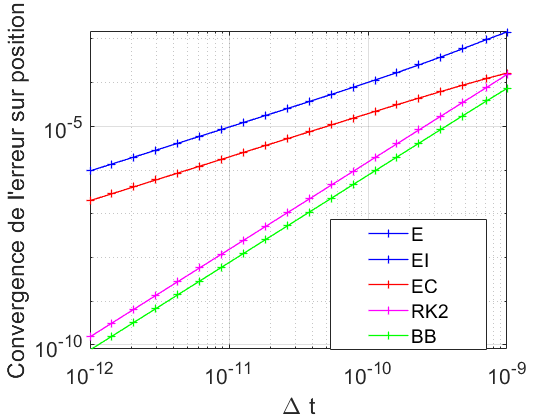
\includegraphics[scale=0.6]{Convergence_erreur_position_tous_integrateurs.png}
				\caption{\em\label{Fig:Convergence erreur position} Convergence de l'erreur sur la position en $\Delta t$}
			\end{minipage}
			\hfill%
			\begin{minipage}[c]{.46\linewidth}
				\centering
				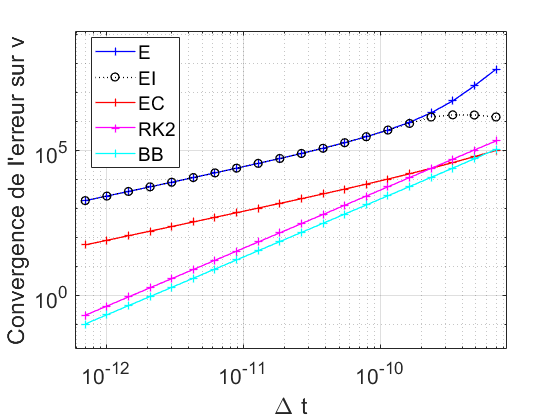
\includegraphics[scale = 0.6]{Convergence_erreur_vitesse_tous_integrateurs.png}
				\caption{\em\label{Fig: Convergence erreur vitesse} Convergence de l'erreur sur la vitesse en $\Delta t$}
			\end{minipage}
		\end{figure}

		Dans la figure \ref{Fig:Convergence erreur position} une simulation de l'erreur maximale locale sur la position a \'et\'e faite. C'est donc l'erreur num\'erique qui est observ\'ee. On repr\'esente les convergences selon les 5 int\'egrateurs : Euler explicite (E), Euler implicite (EI), Euler-Cromer (EC), Runge-Kutta d'ordre 2 (RK2) et Boris-Buneman (BB). On s'int\'eresse maintenant \`a leur ordre de convergence, ce dernier est d\'efini ici comme \'etant la pente de la courbe form\'ee par l'erreur lorsque $\Delta t$ est petit. Une fonction a \'et\'e cr\'e\'ee dans le fichier Parameterscan pour calculer ces pentes. Les résultats sont les suivants.
		
		Pour Euler implicite, les ordres de convegence de la position et de la vitesse sont les m\^emes et valent 1. Il en va de m\^eme pour Euler implicite.
		
		Euler-Cromer est \'egalement d'ordre 1 pour la position et la vitesse, ce qui se confirme par la figure \ref{Fig:Convergence erreur position} car on voit que les trois droites des premiers int\'egrateurs sont parall\`eles. 
		
		Runge-Kutta et Boris-Buneman sont d'ordre 2, ce qui est confirmé par les deux droites parall\`eles sur la figure \ref{Fig: Convergence erreur vitesse}.
		
		
		
		

		\subsubsection{Non-conservation de l'Energie m\'ecanique}
		
		
	\begin{figure}[h]
		\begin{minipage}[c]{.46\linewidth}
			\centering
			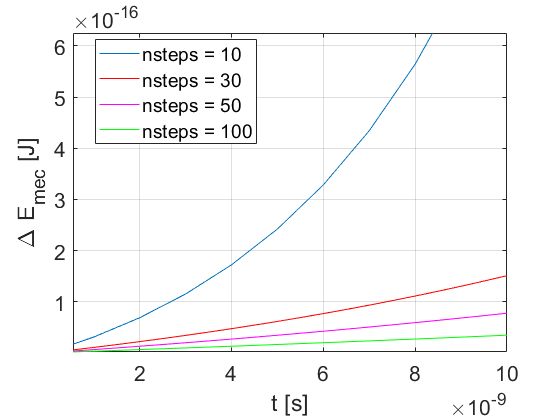
\includegraphics[scale = 0.6]{D_E_mec_E.png}
			\caption{\em\label{Fig:Emec E} Variation de l'\'energie m\'ecanique selon Euler explicite en $\Delta t$}
		\end{minipage}
		\hfill%
		\begin{minipage}[c]{.46\linewidth}
			\centering
			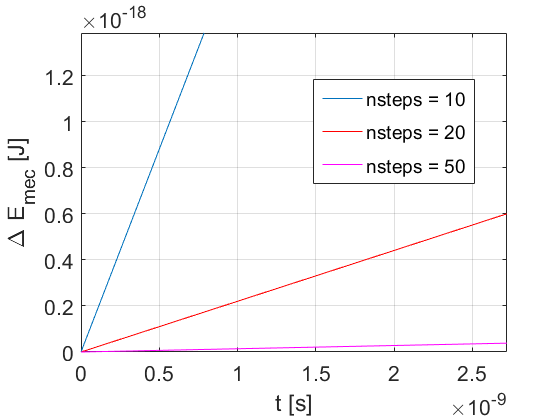
\includegraphics[scale = 0.6]{D_E_mec_RK2.png}
			\caption{\em\label{Fig: Emec RK2} Variation de l'\'energie m\'ecanique selon Runge-Kutta 2 en $\Delta t$}
		\end{minipage}
	\end{figure}

		La figure \ref{Fig:Emec E} montre que l'int\'egrateur d'Euler explicite est instable car, pour des petits pas de temps, on voit clairement que $\Delta E_{mec}$ croît exponentiellement. 
		En ce qui concerne Runge-Kutta, on voit sur la figure \ref{Fig: Emec RK2} que la variation de l'\'energie m\'ecanique croît fortement pour des petits pas de temps, elle est donc \'egalement instable.
		
				\begin{figure}[h]
				\begin{minipage}[c]{.46\linewidth}
					\centering
					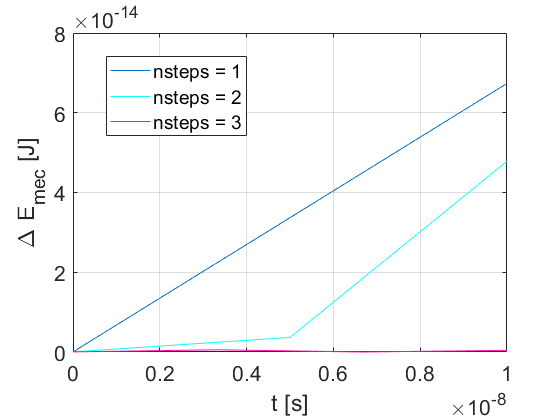
\includegraphics[scale = 0.6]{D_E_mec_EC_n=1_2_3.png}
					\caption{\em\label{Fig:Emec EC} Variation de l'\'energie m\'ecanique selon Euler-Cromer en $\Delta t$ pour des petits nombres de pas }
				\end{minipage}
				\hfill%
				\begin{minipage}[c]{.46\linewidth}
					\centering
					\includegraphics[scale = 0.6]{D_E_mec_Ec_n=10_20_50_100.png}
					\caption{\em\label{Fig: Emec ECC} Variation de l'\'energie m\'ecanique selon Euler-Cromer en $\Delta t$ pour des plus grands nombres de pas}
				\end{minipage}
			\end{figure}
		
		Dans la figure \ref{Fig:Emec EC}, qui concerne l'int\'egrateur d'Euler-Cromer, il est observable qu'avec un pas de temps de 3 l'\'energie est conserv\'ee, alors que si il est plus petit que 3, l'\'energie m\'ecanique n'est pas conserv\'ee. Cela est d\^u au fait qu'Euler-Cromer n'est stable que si $w_c \delta t <2$. Avec $w_c = \frac{qB_0}{m}$, la vitesse de rotation du proton. Ce qui donne le nombre de pas limite $n > 2.3948$, ce qui est bien visible dans la figure \ref{Fig:Emec EC}.
		
		Dans le graphique \ref{Fig: Emec ECC}, on voit que plus le pas de temps est grand, plus l'\'energie est bien conserv\'ee, la courbe oscille autour de 0 et montre donc que c'est un sch\'ema stable quand le pas de temps minimum est respect\'e.
		
		\begin{figure}[h]
			\begin{minipage}[c]{.46\linewidth}
				\centering
				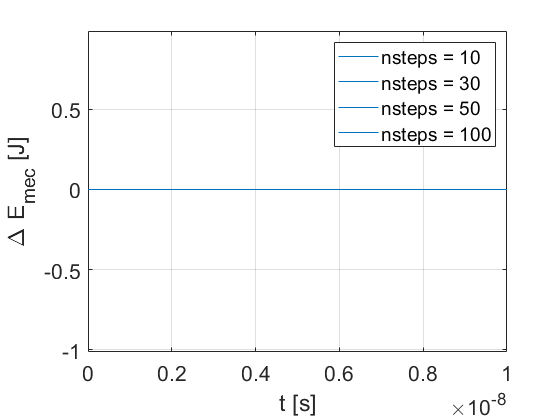
\includegraphics[scale = 0.6]{D_E_mec_BB.png}
				\caption{\em\label{Fig:Emec BB} Variation de l'\'energie m\'ecanique selon Boris Buneman en $\Delta t$ }
			\end{minipage}
			\hfill%
			\begin{minipage}[c]{.46\linewidth}
				\centering
				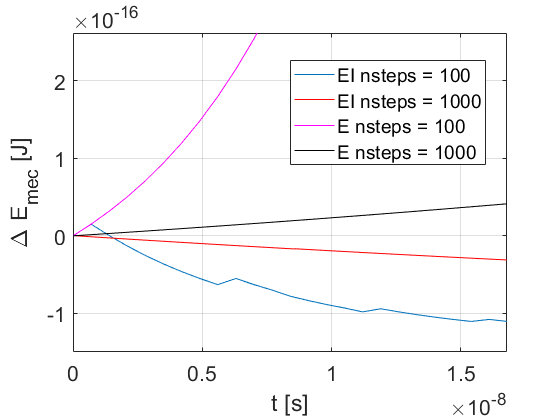
\includegraphics[scale = 0.6]{D_E_mec_EI.png}
				\caption{\em\label{Fig: Emec EI2} Variation de l'\'energie m\'ecanique selon Euler implicite et Euler explicite  en $\Delta t$}
			\end{minipage}
		\end{figure}
	
	La figure \ref{Fig:Emec BB} montre que l'int\'egrateur de Boris-Buneman conserve exactement l'\'energie m\'ecanique, aux arrondis pr\`es, pour tous les pas de temps et, par cons\'equent, pour toute valeur de $\Delta t$.
	
	Et la figure \ref{Fig: Emec EI2} est faite  afin de pouvoir comparer les deux int\'egrateurs d'Euler explicite et implicite. On voit nettement que le sch\'ema implicite est bien plus stable que l'explicite, cependant il d\'cro\^it contrairemtn \`a l'autre. Cela est d\^u au fait qu'il dissipe de l'\'energie, ce qui est ce \`a quoi on s'attend, comme dit dans le polycopi\'e (\cite{NdC}, p.34). Cette dissipation est d'origine num\'erique et non pas physique.
		
	
\subsection{Cas avec un champ \'electrique et un champ magn\'etique : d\'erive $\Vec{E}\times\Vec{B}$}
Dans cette partie il est consider\'e que la valeur $E_0 \ne 0$, mais que $E_0 = 10^5$Vm$^{-1}$. Les autres valeurs restent comme dans l'exercice pr\'ec\'edent. Les sch\'emas utilis\'ees sont Runge-Kutta d'ordre 2 et Boris-Buneman.
	\subsubsection{\'Etude de convergence en $\Delta t$}
	En impl\'ementent les solutions analytiques dans le fichier ParameterScan.m de Matlab, la figure obtenu pour le maximum de l'erreure de la position en fonction de $\Delta t$. Nous obtenons des droites pour Runge-Kutta d'ordre 2 et pour Boris-Buneman, que l'on peut observer sur la figure \ref{Fig: Conv Pos}, ce qu'implique une convergence lin\'eaire en fonction de $\Delta t$. En utilisant un fit lin\'eaire on peut d\'eterminer l'ordre de convergence des deux sch\'emas, qui est 2 ($y = 2x + 32$ et $y = 2x + 32.5$), facilement v\'erifiable sur la figure \ref{Fig: Fit Lin Pos}.
	
	
	\begin{figure}[h]
				\begin{minipage}[c]{.46\linewidth}
					\centering
					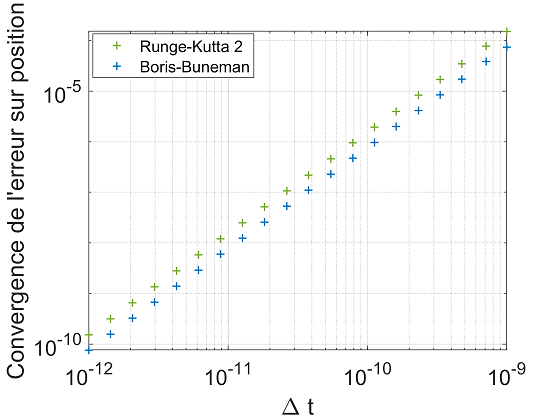
\includegraphics[scale = 0.6]{conv_pos_RK_BB.png}
					\caption{\em\label{Fig: Conv Pos} Etude de la convergence de l'erreure maximale sur la position selon $\Delta t$}
				\end{minipage}
				\hfill%
				\begin{minipage}[c]{.46\linewidth}
					\centering
					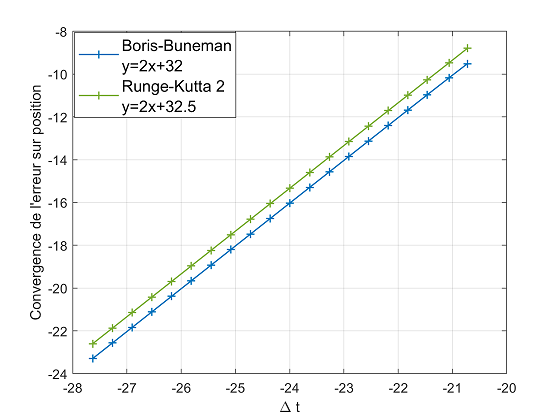
\includegraphics[scale = 0.6]{fit_lin_pos.png}
					\caption{\em\label{Fig: Fit Lin Pos} Fit lin\'eaire de l'erreure sur la position en $\Delta t$}
				\end{minipage}
			\end{figure}
			
			
	\subsubsection{Conservation de l'\'energie}
	En prenons en compte le champ \'el\'ectrique, nous avons une nouvelle force \`a considerer. La charge $q$ de la particule \'etant positive, on a $\Vec{F_E} = qE_0\Vec{e_z}$, et donc la force est orient\'e comme le champ \'el\'ectrique, ce qu'implique que l'\'energie potentielle est n\'egative selon l'axe $\Vec{e_z}$ d'apr\`es la formule $\Vec{E} = -\int \Vec{F}d\Vec{z}$. On peut donc exprimer l'\'energie m\'ecanique comme : 
	\begin{equation}\label{e_m_b_ii}
	E_{mec} = \frac{1}{2}m\left|\left|\Vec{v}\right|\right|^2 - qEz
	\end{equation}
	En d\'efinissont $\Delta E(t)$ comme $E(t)$ et $E(0)$, on fait une \'etude de convergence de $\Delta E(t)$ en fonction de nombre de pas (nsteps). Ceci est repr\'esent\'ee sur la fig \ref{Fig: }.
	
	\begin{figure}[h]
					\centering
					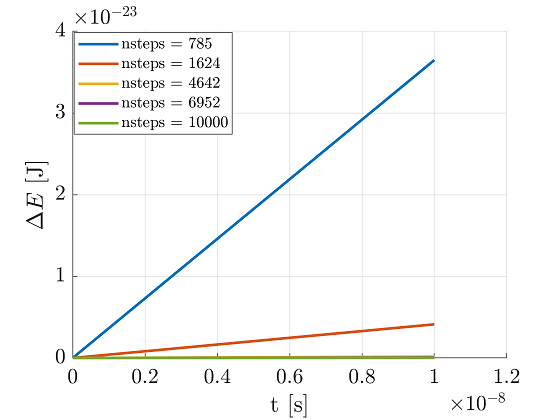
\includegraphics[scale = 0.6]{ener_mec_cons.png}
					\caption{\em\label{Fig: Cons Emec} $\Delta E(t)$ en fonction du nombre de pas de temps.}
	\end{figure}
On n'arrive pratiquement pas \`a diff\'erencier les droites pour les valeurs : $n_{steps} = 4642$, $n_{steps} = 6952$ et $n_{steps} = 10000$, mais on arrive bien \`a voir que la valeur de $\Delta E(t)$ semble bien converger lorsque $n_{steps}$ devient grand :

\begin{equation}\label{cons_en}
\lim_{n_{steps} \rightarrow +\infty} \Delta E(t) = 0 \forall t \in [0;t_{fin}]
\end{equation}

\subsubsection{Trajectoire de la particule dans un r\'ef\'erentiel en translation uniforme \`a la vitesse $v_E = \Vec{E}\times\Vec{B}/B^2$}

La formule de $v_E$ \'etant donn\'e, on peut calculer sa valeur, qui est donn\'e par : 
\begin{equation}\label{v_e}
\Vec{v}_E = \frac{1}{B_0^2}\begin{pmatrix}0 \\ 0 \\ E_0 \end{pmatrix}\times\begin{pmatrix}0 \\ B_0 \\ 0 \end{pmatrix} = -\frac{1}{B_0}\begin{pmatrix}E_0 \\ 0 \\ 0 \end{pmatrix}
\end{equation}

On peut soustraire la valeur dans l'\'equation de $v_x(t)$ de l'\'equation \ref{sol_an}, ce qui donne :
\begin{equation}\label{sol v_e}
v_x(t) = - v_0\sin(\frac{qB_0}{m}t) + \frac{E_0}{B_0}\cos(\frac{qB_0}{m}t)
\end{equation}



\subsection{Cas d'un champ magn\'etique non uniforme : d\'erive $\Vec{B}\times\nabla B$}
Dans cette section nous consid\'erons un champ magn\'etique d'intensit\'e variable $\Vec{B} = B(x)\hat{y}$, o\`u $B(x) = B_0(1 + \kappa x)$, $\kappa = 100$m$^{-1}$, $B_0 = 5$T, $E = 0$, $v_{x_0} = 0$, $v_{z_0} = 4\cdot10^5$m.s$^{-1}$, $x_0 = \frac{mv_{z_0}}{qB_0}$, $z_0 = 0$ et $t_{fin} = 6.5593\cdot10^{-7}$s. Le sch\'ema utilis\'e est Boris-Buneman.

\subsubsection{Cas d'un proton ($q = e$) et d'un antiproton ($q = -e$)}
Dans les cas de proton et antiproton les trajectoires sont des cyclo\"\i des, et on peut observer que lorsque $n_{steps}$ devient tr\`es grand, leurs orbites deviennent de plus en plus des colonnes droites. On peut voir leurs limites sur les figures \ref{Fig: Prot Traj} et \ref{Fig: Anti Traj}.
\begin{figure}[h]
				\begin{minipage}[c]{.46\linewidth}
					\centering
					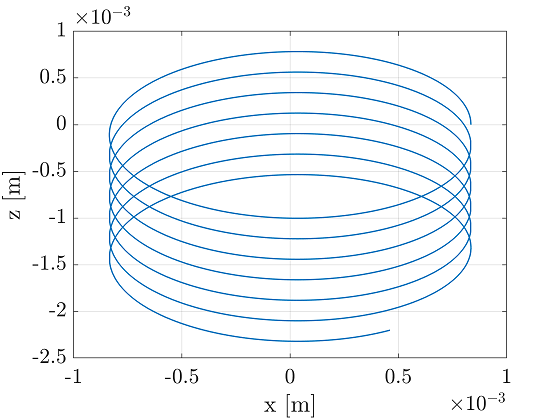
\includegraphics[scale = 0.6]{final_traj_prot.png}
					\caption{\em\label{Fig: Prot Traj} Trajectoire d'un proton.}
				\end{minipage}
				\hfill%
				\begin{minipage}[c]{.46\linewidth}
					\centering
					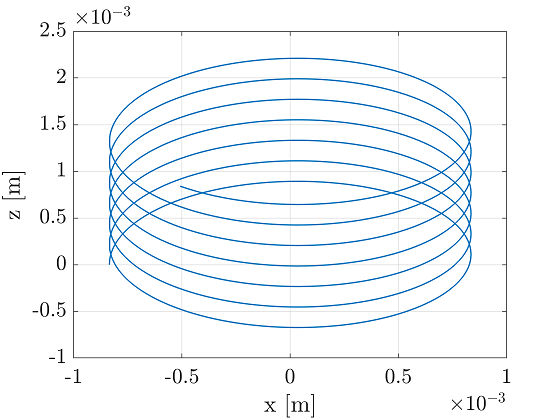
\includegraphics[scale = 0.6]{final_traj_antiprot.png}
					\caption{\em\label{Fig: Anti Traj} Trajectoire d'un antiproton.}
				\end{minipage}
			\end{figure}
On voit que la colonne du proton est orient\'e vers le bas, alors que celui de l'antiproton est orient\'e vers le haut. La trajectoire est parcourue dans un sens anti-horaire par le proton, et dans un sens horaire par l'antiproton.

\subsubsection{La quantit\'e $\mu = \frac{mv^2}{2B}$}
La quantit\'e $\mu$ s'appelle le moment magn\'etique d'une particule, dans notre cas soit du proton, soit de l'antiproton. Il caract\'erise l'intensit\'e de la source magn\'etique. L'\'enconc\'e \cite{Notes} nous dit que $B(x) = B_0(1 + \kappa x) = B_0 + B_0x\kappa$. Il est \'evident que cette fonction d\'epend en entier de la valeur de $x$, et a donc des extremas en fonction des extremas de la fonction $f(x) = x$. Sur les figures suivantes, o\`u les positions des particules et les valeurs des moments magn\'etiques des particules sont repr\'esent\'ees sur un intervalle de temps de $\Delta t = 1\times 10^{-7}$, pour qu'on puisse voir avec plus de pr\'ecision ce que se passe, on voit que $\mu$ est inversement proportionnel \`a la position de la particule.

\begin{figure}
\begin{minipage}[c]{.46\linewidth}
					\centering
					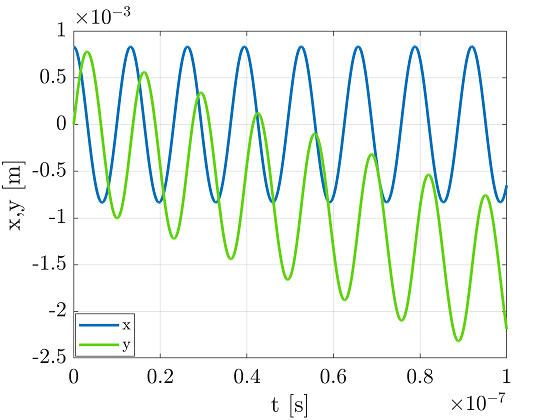
\includegraphics[scale = 0.6]{proton_pos.png}
					\caption{\em\label{Fig: Pos Prot} Position du proton.}
				\end{minipage}
				\hfill%
				\begin{minipage}[c]{.46\linewidth}
					\centering
					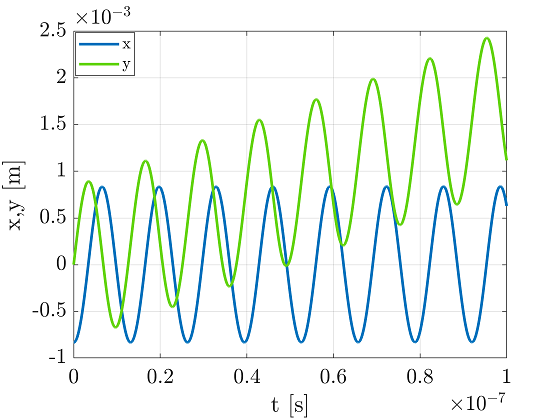
\includegraphics[scale = 0.6]{antiproton_pos.png}
					\caption{\em\label{Fig: Pos Anti} Position du antiproton.}
				\end{minipage}
			\end{figure}
		
\begin{figure}
\begin{minipage}[c]{.46\linewidth}
					\centering
					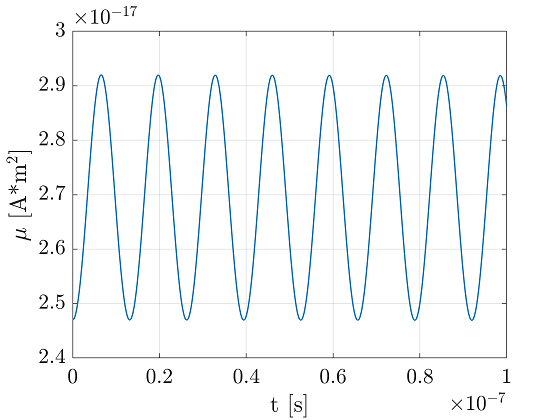
\includegraphics[scale = 0.6]{mm_p.png}
					\caption{\em\label{Fig: mm Prot} Moment magn\'etique du proton.}
				\end{minipage}
				\hfill%
				\begin{minipage}[c]{.46\linewidth}
					\centering
					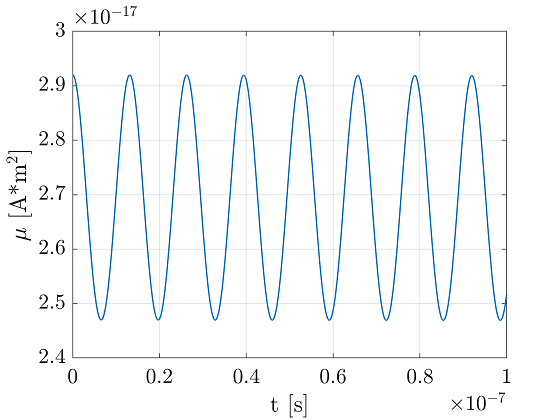
\includegraphics[scale = 0.6]{mm_ap.png}
					\caption{\em\label{Fig: mm Anti} Moment magn\'etique du antiproton.}
				\end{minipage}
			\end{figure}





\section{Conclusions}



%-----------------------------------------------------------


\begin{thebibliography}{99}
 \bibitem{NdC}
 L. Villard avec la contribution de A. L\"auchli {\it Notes de cours Physique numérique I-II, version 20.1} (2020)
 
 \bibitem{Notes}
 L. Villard, Dr C. Sommariva {\it \'Enonc\'e de l'exercice 2} (2020)
 \url{https://moodle.epfl.ch/pluginfile.php/2839539/mod_resource/content/1/Exercice2_2020.pdf}
 
 \bibitem{FT}
 VEREIN SCHWEIZERISCHER MATHEMATIK- UND PHYSIKLEHRER  et al. {\it Formulaires et tables : mathématiques, physique, chimie} Editions G d'Encre, 2015. ISBN 978-2-940501-41-0
 
\end{thebibliography}

\end{document} %%%% THE END %%%%
